\section{Appendix for MS1}

\begin{figure}[H]
    \centering
    \subfloat[Validation Set]{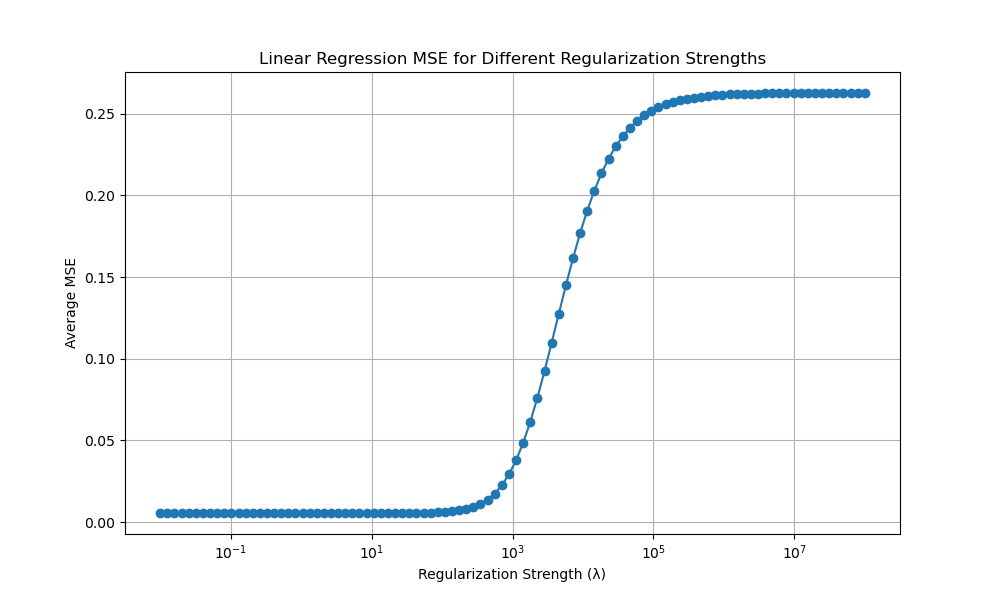
\includegraphics[width=0.4\textwidth]{images/linear_regression_lambda.png}}
    \hfill
    \subfloat[5-Fold Cross Validation]{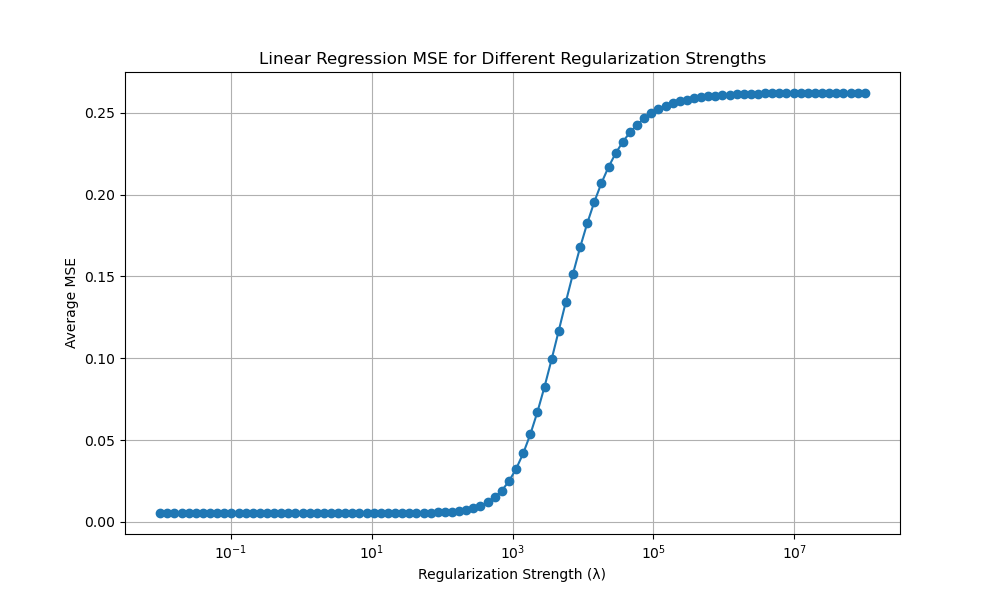
\includegraphics[width=0.4\textwidth]{images/linear_regression_lambda_k_fold.png}}
    \caption{Graphs showing best lambda's using validation set or 5-fold cross validation}
    \label{fig:images}
  \end{figure}

\begin{figure}[H]
  \centering
  \subfloat[lr from 0.001 to 0.01]{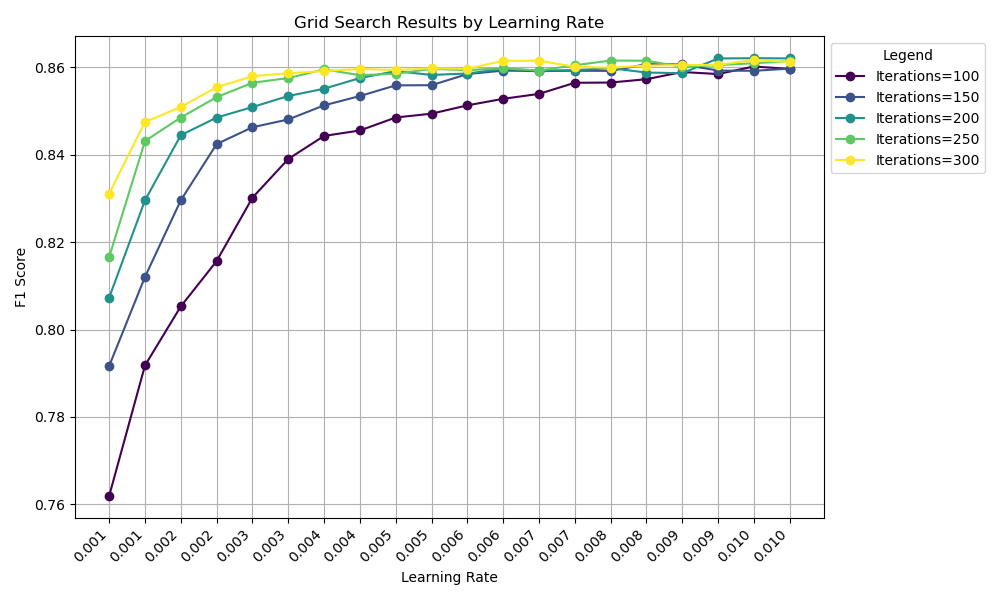
\includegraphics[width=0.4\textwidth]{images/grid_search_to_0_2.png}\label{fig:f4}}
  \hfill
  \subfloat[lr from 0.01 to 0.1]{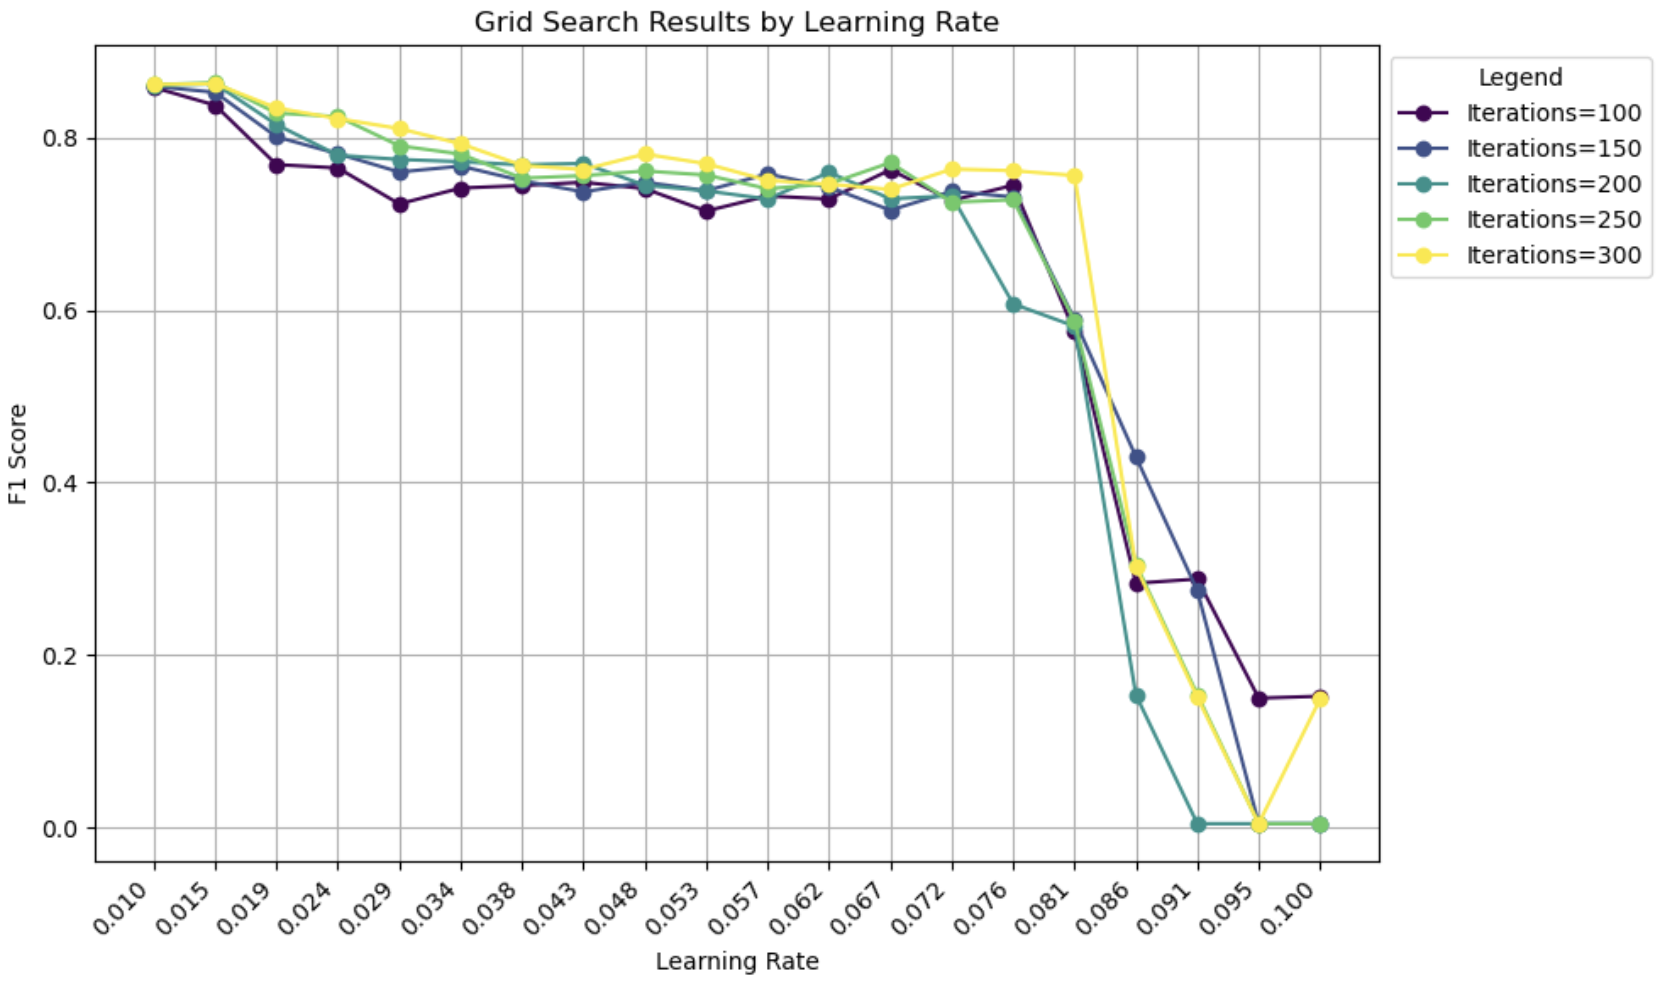
\includegraphics[width=0.4\textwidth]{images/grid_search_to_0_1.png}\label{fig:f5}}
  \caption{Graphs clearly showing that the best learning rate are between 0.01 and 0.015 with 300 hundred iterations}
  \label{fig:images2}
\end{figure}

\begin{figure}[H]
  \centering
  \subfloat[K from 1 to 30]{\includegraphics[width=0.4\textwidth]{images/knn\_k\_values1.png}\label{fig:f1}}
  \hfill
  \subfloat[K from 1 to 2500]{\includegraphics[width=0.4\textwidth]{images/knn\_k\_values.png}\label{fig:f2}}
  \caption{Graphs clearly showing that as K increases the MSE tends to an asymptotic value when center\_locating}
  \label{fig:images3}
\end{figure}

\imagehere[0.5]{./images/knn\_k\_values2.png}{Graph showing the best K value for the KNN algorithm breed\_identifying}{fig:image4}


